\documentclass[preview]{standalone}
%\usepackage{prelude}

%%%%%%%%%%%%%%%%%%%%%%%%%%%%%%%%%%%% PACKAGES %%%%%%%%%%%%%%%%%%%%%%%%%%%%%%%%%%%%%%%%%%

\usepackage{inputenc,fontenc}
\usepackage[a4paper,margin=3cm]{geometry}
\usepackage[english]{babel}
%\usepackage[german]{babel}
%\usepackage[fixlanguage]{babelbib}


\usepackage{bbold}
\usepackage{amsthm}
\usepackage{amsmath}
\usepackage{amssymb} % doteqdot
\usepackage[dvipsnames]{xcolor}
\usepackage{standalone}
\usepackage{tikz}[mode=buildnew]
\usepackage{cite}
\usepackage{xspace}
\usepackage{relsize}
\usepackage{mathtools} % mathclap
%\usepackage{MnSymbol}
\usepackage{hyperref}
\usepackage{url}
\usepackage{listings} % for code
\usepackage[T1]{fontenc} %<
\hypersetup{
	colorlinks,
	citecolor=black,
	filecolor=black,
	linkcolor=black,
	urlcolor=black
}
\usepackage{pgfplots}
\pgfplotsset{compat=1.18}
%\usepackage{courier} %% Sets font for listing as Courier. But also for url and texttt!
\usepackage{listings, xcolor}
\usepackage{graphicx}
\usepackage{subcaption}

\usetikzlibrary{calc}
%\usepackage{xparse} % \newDocumentCommand for multiple optional arguments
%\usepackage{titlecaps}



%%%%%%%%%%%%%%%%%%%%%%%%%%%%%%%%%%%% THEOREMSTYLES %%%%%%%%%%%%%%%%%%%%%%%%%%%%%%%%%%

\theoremstyle{definition}
\newtheorem{definition}{Definition}[section]
\newtheorem{exmp}{Beispiel}[section]
%\AfterEndEnvironment{definition}{\noindent\ignorespaces}

\theoremstyle{theorem}
\newtheorem{theorem}{Satz}[section]
\newtheorem{proposition}{Proposition}[section]
%\AfterEndEnvironment{theorem}{\noindent\ignorespaces}

\theoremstyle{korollary}
\newtheorem{korollary}{Korollar}[section]
%\AfterEndEnvironment{korollary}{\noindent\ignorespaces}


\tikzset{
	mstate/.style={draw, circle, minimum size=.94cm}, 
	gstate/.style={draw, rectangle, minimum size=.8cm},
	varstate/.style={draw,rectangle, rounded corners, minimum size=1}, 
	trans/.style={draw, ->, thick},
	bendtrans/.style={draw, ->, thick, bend left=10},
	bendtransr/.style={draw, ->, thick, bend right=10},
	init/.style={initial, initial distance=6pt, initial text=},
	every loop/.style={min distance=5pt, looseness=8},
	>=latex
}
\usetikzlibrary{automata,positioning}

%auto shift/.style={auto=right,->,
%	to path={ let \p1=(\tikztostart),\p2=(\tikztotarget),
%		\n1={atan2(\y2-\y1,\x2-\x1)},\n2={\n1+180}
%		in ($(\tikztostart.{\n1})!1mm!270:(\tikztotarget.{\n2})$) -- 
%		($(\tikztotarget.{\n2})!1mm!90:(\tikztostart.{\n1})$) \tikztonodes}},

%%%%%%%%%%%%%%%%%%%%%%%%%%%%%%%%%%% MY MACROS %%%%%%%%%%%%%%%%%%%%%%%%%%%%%%%%%%%%%%%%%
%formatting
\newcommand{\comment}[2]{{\color{#1}#2}}
\newcommand{\redcomment}[1]{{\color{red}#1}}
\newcommand{\purpcomment}[1]{{\color{pink}#1}}
\newcommand{\bluecomment}[1]{{\color{blue}#1}}
\newcommand{\mt}[1]{\ensuremath{{#1}}\xspace}
\newcommand{\mynewcommand}[2]{\newcommand{#1}{\mt{#2}}} %% currently not used becaue of ide highlighting
\newcommand{\arr}{\mt{\to}}

%model checking terms
\newcommand{\mimicrel}{\mt{\mathcal{R}}}
\newcommand{\bisimeq}{\mt{\;\!\sim\;\!}}
\newcommand{\simorder}{\mt{\;\!\preceq\;\!}}
\newcommand{\simequiv}{\mt{\;\!\simeq\;\!}} %command already defined
\newcommand{\relts}{\mt{\;\!\bullet_{_{\tiny{TS}}}\;\!}}
\newcommand{\rel}{\mt{\;\!\bullet\;\!}}

%own names
\newcommand{\nm}[1]{#1\xspace}
\newcommand{\mdpN}{\nm{MDP}}
\newcommand{\mdpsN}{\nm{MDPs}}
\newcommand{\viewN}{\nm{view}}
\newcommand{\viewNC}{\nm{View}}
\newcommand{\viewsN}{\nm{views}}
\newcommand{\viewsNC}{\nm{Views}}
\newcommand{\grpfctsubN}{\nm{detached grouping function}}
\newcommand{\grpfctsubNC}{\nm{detached grouping function}}
\newcommand{\grpfctsubNCC}{\nm{Detached Grouping Function}}
\newcommand{\grpfctN}{\nm{grouping function}}
\newcommand{\grpfctNC}{\nm{Grouping function}}
\newcommand{\grpfctNCC}{\nm{Grouping Function}}
\newcommand{\grpfctsN}{\nm{grouping functions}}
\newcommand{\grpfctsNC}{\nm{Grouping functions}}
\newcommand{\grpfctsNCC}{\nm{Grouping Functions}}
\newcommand{\stmimicN}{\nm{state-mimic}}
\newcommand{\stmimicsN}{\nm{state-mimics}}
\newcommand{\stmimickingN}{\nm{state-mimicking}}
\newcommand{\stmimickedN}{\nm{state-mimicked}}
%\newcommand{\chosenphtypeNCC}{\nm{Transition System}}
%\newcommand{\chgphNC}{\nm{Transition system}}
%\newcommand{\chgphN}{\nm{transition system}}
%\newcommand{\chgphsNCC}{\nm{Transition Systems}}
%\newcommand{\chgphsNC}{\nm{Transition systems}}
%\newcommand{\chgphsN}{\nm{transition systems}}
\newcommand{\chgphNCC}{\nm{MDP}}
\newcommand{\chgphNC}{\nm{MDP}}
\newcommand{\chgphN}{\nm{MDP}}
\newcommand{\achgphN}{\nm{an MDP}}
\newcommand{\chgphsNCC}{\nm{MDPs}}
\newcommand{\chgphsNC}{\nm{MDPs}}
\newcommand{\chgphsN}{\nm{MDPs}}
\newcommand{\parllcompN}{\nm{parallel composition}}
\newcommand{\parllcompNC}{\nm{Parallel composition}}
\newcommand{\parllcompNCC}{\nm{Parallel Composition}}
\newcommand{\parllcompsN}{\nm{parallel compositions}}
\newcommand{\parllcompsNC}{\nm{Parallel compositions}}
\newcommand{\parllcompsNCC}{\nm{Parallel Compositions}}
\newcommand{\sccN}{\nm{SCC}}
\newcommand{\sccsN}{\nm{SCCs}}
\newcommand{\bsccN}{\nm{BSCC}}
\newcommand{\bsccsN}{\nm{BSCCs}}
\newcommand{\jgrapht}{\nm{jGraphtT}}

\newcommand{\outactident}{\nm{OutActionsIdent}}

%names
\newcommand{\iffN}{\nm{if and only if}}
\newcommand{\tsN}{\nm{TS}}

%% outactions identical
\newcommand{\outactidentstrong}{\nm{strong}}
\newcommand{\outactidentweak}{\nm{weak}}

% CORE DEFINITIONS
\newcommand{\grpfct}[1][\viewppty]{\mt{F_{#1}}}
\newcommand{\grpfctsub}[1][\viewppty]{\mt{\tilde{F}_{#1}}}
%\newcommand{\grpfctimg}[1]{\mt{{\grpfct}[{#1}]}}
%\newcommand{\fctimg}[2]{\mt{{#1}[{#2}]}}
\newcommand{\eqrelview}{\mt{R}}
\newcommand{\eqclassv}[1][\state]{\mt{\eqclass{#1}{\eqrelview}}}
\newcommand{\eqclasssetv}[1][\states]{\mt{{#1}/\eqrelview}} %OLD: \bigcup_{\state \in \states} \eqclassv
\newcommand{\viewid}{\mt{\mdp}}
\newcommand{\view}[1][\viewppty]{\mt{\viewid_{#1}}}
\newcommand{\imggrp}{\mt{\arbset}}
\newcommand{\imggrpsub}{\mt{X}}
\newcommand{\viewppty}{\mt{\theta}}
\newcommand{\pll}{\mt{\;\!\pllpure\;\!}}
\newcommand{\pllrev}{\mt{\pllpure^{-1}}}
\newcommand{\pllpure}{\mt{||}}
\newcommand{\compselectset}{\mt{Z}}
\newcommand{\compselectpure}{\mt{\pllpure_\compselectset}}
\newcommand{\compselect}{\mt{\;\pllpure_\compselectset\;}}
\newcommand{\remstates}{\mt{\bigcup_{\state \in \states \setminus \states_1}\{\{\state\}\}}}
\newcommand{\nogroupstates}[1][\states_2]{\mt{\bigcup_{\state \in \states \setminus {#1}}\{\{\state\}\}}}
\newcommand{\remelem}{\mt{\bullet}}
\newcommand{\nogroupset}{\mt{\xi}}
\newcommand{\remset}{\mt{\{\remelem\}}}
\newcommand{\gfctpll}{\mt{\grpfct[\pll]}}
\newcommand{\group}{\mt{\top}}
\newcommand{\imggrpbinview}{\mt{\{\remelem, \notppty\}}}
\newcommand{\viewappset}{\mt{\tilde{\states}}}
\newcommand{\hasppty}{\mt{\top}}
\newcommand{\notppty}{\mt{\bot}}
\newcommand{\disregardelem}{\mt{\Delta}}
\newcommand{\disregardelements}{\mt{{\disregardelem_1, \dots, \disregardelem_n}}}



%\newcommand{\mdp}{def}\mdp
%\newcommand{\mdpdef}



% EXAMPLE VIEWS
\newcommand{\pptyatomicprops}{\mt{\atomicprops}}
\newcommand{\pptyinitstates}{\mt{\initstates}}
\newcommand{\pptyinactsetsize}{\mt{|\inacts(\state)|}}
\newcommand{\pptyhasoutact}{\mt{\exists\outact}}
\newcommand{\pptyminoutact}[2]{\mt{#1\leq#2}}
\newcommand{\pptymaxoutact}[2]{\mt{#2\leq#1}}
\newcommand{\pptyspanoutact}[3]{\mt{#1\leq#2\leq#3}}
\newcommand{\pptyoutactsetsize}{\mt{|\outacts(\state)|}}
\newcommand{\pptyoutactsingle}{\mt{|\outacts(\state)|_1}}
\newcommand{\pptystrongoutactident}{\mt{\outacts(\state)_=}}
\newcommand{\pptyweakoutactident}{\mt{\outacts(\state)_\approx}}
\newcommand{\pptyhasinact}{\mt{\exists\inact}}
\newcommand{\pptymininact}[2]{\mt{#1\leq#2}}
\newcommand{\pptymaxinact}[2]{\mt{#2\leq#1}}
\newcommand{\pptyspaninact}[3]{\mt{#1\leq#2\leq#3}}
\newcommand{\pptyinactsingle}{\mt{|\inacts(\state)|_1}}
\newcommand{\pptystronginactident}{\mt{\inacts(\state)_=}}
\newcommand{\pptyweakinactident}{\mt{\inacts(\state)_\approx}}
\newcommand{\pptyparamvalueseq}{\mt{\var = \varval}}
\newcommand{\pptyparamvaluesneq}{\mt{\var \neq \varval}}
\newcommand{\pptyparamdnf}{\mt{VarDNF}}
\newcommand{\pptyparamcnf}{\mt{VarCNF}}
\newcommand{\pptyparamvalueseqopt}{\mt{\var = \varval}}
\newcommand{\pptyparamvalident}{\mt{Var:\varval}}
\newcommand{\pptydistance}{\mt{\distpath}}
\newcommand{\pptydistancerev}{\mt{\distpathrev}}
\newcommand{\pptydistancebi}{\mt{\distpathbi}}
\newcommand{\pptyhascycle}{\mt{\exists\cycle}}
\newcommand{\pptyexactactcycle}{\mt{\{\cycle_{\action,n}\}}}
\newcommand{\pptycycleset}{\mt{\cup{\{\state\}_\cycle}}}
\newcommand{\pptyexactcycle}{\mt{\{\cycle_n\}}}
\newcommand{\pptyscc}{\mt{scc}}
\newcommand{\pptybscc}{\mt{bscc}}
\newcommand{\pptyprop}{\mt{\redcomment{?}}}
\newcommand{\pptyident}{id}


\newcommand{\gfctatomicprops}{\mt{\grpfct[\pptyatomicprops]}}
\newcommand{\gfctinitstates}{\mt{\grpfct[\pptyinitstates]^\hasppty}}
\newcommand{\gfcthasoutaction}{\mt{\grpfct[\pptyhasoutact]^\hasppty}}
\newcommand{\gfctminoutaction}{\mt{\grpfct[\pptyminoutact{\numoutact}{\outact}]^\hasppty}}
\newcommand{\gfctmaxoutaction}{\mt{\grpfct[\pptymaxoutact{\numoutact}{\outact}]^\hasppty}}
\newcommand{\gfctspanoutaction}{\mt{\grpfct[\pptyspanoutact{\numoutactb}{\outact}{\numoutact}]^\hasppty}}
\newcommand{\gfctoutactsetsize}{\mt{\grpfct[\pptyoutactsetsize]}}
\newcommand{\gfctoutactsingle}{\mt{\grpfct[\pptyoutactsingle]^\notppty}}
\newcommand{\gfctstrongoutactident}{\mt{\grpfct[\pptystrongoutactident]}}
\newcommand{\gfctweakoutactident}{\mt{\grpfct[\pptyweakoutactident]}}
\newcommand{\gfcthasinaction}{\mt{\grpfct[\pptyhasinact]^\hasppty}}
\newcommand{\gfctmininaction}{\mt{\grpfct[\pptymininact{\numinact}{\inact}]^\hasppty}}
\newcommand{\gfctmaxinaction}{\mt{\grpfct[\pptymaxinact{\numinact}{\inact}]^\hasppty}}
\newcommand{\gfctspaninaction}{\mt{\grpfct[\pptyspaninact{\numinactb}{\inact}{\numinact}]^\hasppty}}
\newcommand{\gfctinactsetsize}{\mt{\grpfct[\pptyinactsetsize]}}
\newcommand{\gfctinactsingle}{\mt{\grpfct[\pptyinactsingle]^\notppty}}
\newcommand{\gfctstronginactident}{\mt{\grpfct[\pptystronginactident]}}
\newcommand{\gfctweakinactident}{\mt{\grpfct[\pptyweakinactident]}}
\newcommand{\gfctparamvalueseq}{\mt{\grpfct[\pptyparamvalueseq]^\hasppty}}
\newcommand{\gfctparamvaluesneq}{\mt{\grpfct[\pptyparamvaluesneq]^\hasppty}}
\newcommand{\gfctparamdnf}{\mt{\grpfct[\pptyparamdnf]^\hasppty}}
\newcommand{\gfctparamcnf}{\mt{\grpfct[\pptyparamcnf]^\hasppty}}
\newcommand{\gfctparamvalueseqopt}{\mt{\pptyparamvalueseqopt}}
\newcommand{\gfctparamvalident}{\mt{\grpfct[\pptyparamvalident]}}
\newcommand{\gfctdistance}{\mt{\grpfct[\pptydistance]}}
\newcommand{\gfctdistancerev}{\mt{\grpfct[\pptydistancerev]}}
\newcommand{\gfctdistancebi}{\mt{\grpfct[\pptydistancebi]}}
\newcommand{\gfcthascycle}{\mt{\grpfct[\pptyhascycle]}}
\newcommand{\gfctexactcycle}{\mt{\grpfct[\pptyexactcycle]}}
\newcommand{\gfctcycleset}{\mt{\grpfct[\pptycycleset]}}
\newcommand{\gfctexactactcycle}{\mt{\grpfct[\pptyexactactcycle]}}
\newcommand{\gfctscc}{\mt{\grpfct[\pptyscc]}}
\newcommand{\gfctbscc}{\mt{\grpfct[\pptybscc]}}
\newcommand{\gfctprop}{\mt{\grpfct[\pptyprop]}}
\newcommand{\gfctident}{\mt{\grpfct[\pptyident]}}

\newcommand{\gfctsubatomicprops}{\mt{\grpfctsub[\pptyatomicprops]}}
\newcommand{\gfctsubinitstates}{\mt{\grpfctsub[\pptyinitstates]^\hasppty}}
\newcommand{\gfctsubhasoutaction}{\mt{\grpfctsub[\pptyhasoutact]^\hasppty}}
\newcommand{\gfctsubminoutaction}{\mt{\grpfctsub[\pptyminoutact{\numoutact}{\outact}]^\hasppty}}
\newcommand{\gfctsubmaxoutaction}{\mt{\grpfctsub[\pptymaxoutact{\numoutact}{\outact}]^\hasppty}}
\newcommand{\gfctsubspanoutaction}{\mt{\grpfctsub[\pptyspanoutact{\numoutactb}{\outact}{\numoutact}]^\hasppty}}
\newcommand{\gfctsuboutactsetsize}{\mt{\grpfctsub[\pptyoutactsetsize]}}
\newcommand{\gfctsuboutactsingle}{\mt{\grpfctsub[\pptyoutactsingle]^\notppty}}
\newcommand{\gfctsubstrongoutactident}{\mt{\grpfctsub[\pptystrongoutactident]^\hasppty}}
\newcommand{\gfctsubweakoutactident}{\mt{\grpfctsub[\pptyweakoutactident]^\hasppty}}
\newcommand{\gfctsubhasinaction}{\mt{\grpfctsub[\pptyhasinact]}}
\newcommand{\gfctsubmininaction}{\mt{\grpfctsub[\pptymininact{\numinact}{\inact}]}}
\newcommand{\gfctsubmaxinaction}{\mt{\grpfctsub[\pptymaxinact{\numinact}{\inact}]}}
\newcommand{\gfctsubspaninaction}{\mt{\grpfctsub[\pptyspaninact{\numinactb}{\inact}{\numinact}]}}
\newcommand{\gfctsubinactsetsize}{\mt{\grpfctsub[\pptyinactsetsize]^\hasppty}}
\newcommand{\gfctsubinactsingle}{\mt{\grpfctsub[\pptyinactsingle]^\notppty}}
\newcommand{\gfctsubstronginactident}{\mt{\grpfctsub[\pptystronginactident]}}
\newcommand{\gfctsubweakinactident}{\mt{\grpfctsub[\pptyweakinactident]}}
\newcommand{\gfctsubparamvalueseq}{\mt{\grpfctsub[\pptyparamvalueseq]^\hasppty}}
\newcommand{\gfctsubparamvaluesneq}{\mt{\grpfctsub[\pptyparamvaluesneq]^\hasppty}}
\newcommand{\gfctsubparamdnf}{\mt{\grpfctsub[\pptyparamdnf]^\hasppty}}
\newcommand{\gfctsubparamcnf}{\mt{\grpfctsub[\pptyparamcnf]^\hasppty}}
\newcommand{\gfctsubparamvalueseqopt}{\mt{\pptyparamvalueseqopt}}
\newcommand{\gfctsubparamvalident}{\mt{\grpfctsub[\pptyparamvalident]}}
\newcommand{\gfctsubdistance}{\mt{\grpfctsub[\pptydistance]}}
\newcommand{\gfctsubdistancerev}{\mt{\grpfctsub[\pptydistancerev]}}
\newcommand{\gfctsubdistancebi}{\mt{\grpfctsub[\pptydistancebi]}}
\newcommand{\gfctsubhascycle}{\mt{\grpfctsub[\pptyhascycle]^\hasppty}}
\newcommand{\gfctsubexactcycle}{\mt{\grpfctsub[\pptyexactcycle]}}
\newcommand{\gfctsubcycleset}{\mt{\grpfctsub[\pptycycleset]}}
\newcommand{\gfctsubexactactcycle}{\mt{\grpfctsub[\pptyexactactcycle]}}
\newcommand{\gfctsubscc}{\mt{\grpfctsub[\pptyscc]}}
\newcommand{\gfctsubbscc}{\mt{\grpfctsub[\pptybscc]}}
\newcommand{\gfctsubprop}{\mt{\grpfctsub[\pptyprop]}}
\newcommand{\gfctsubident}{\mt{\grpfctsub[\pptyident]}}


\newcommand{\viewatomicprops}{\mt{\view[\pptyatomicprops]}}
\newcommand{\viewinitstates}{\mt{\view[\pptyinitstates]^\hasppty}}
\newcommand{\viewhasoutaction}{\mt{\view[\pptyhasoutact]^\hasppty}}
\newcommand{\viewminoutaction}{\mt{\view[\pptyminoutact{\numoutact}{\outact}]^\hasppty}}
\newcommand{\viewmaxoutaction}{\mt{\view[\pptymaxoutact{\numoutact}{\outact}]^\hasppty}}
\newcommand{\viewspanoutaction}{\mt{\view[\pptyspanoutact{\numoutactb}{\outact}{\numoutact}]^\hasppty}}
\newcommand{\viewoutactsetsize}{\mt{\view[\pptyoutactsetsize]}}
\newcommand{\viewoutactsingle}{\mt{\view[\pptyoutactsingle]^\notppty}}
\newcommand{\viewstrongoutactident}{\mt{\view[\pptystrongoutactident]}}
\newcommand{\viewweakoutactident}{\mt{\view[\pptyweakoutactident]}}
\newcommand{\viewhasinaction}{\mt{\view[\pptyhasinact]^\hasppty}}
\newcommand{\viewmininaction}{\mt{\view[\pptymininact{\numinact}{\inact}]^\hasppty}}
\newcommand{\viewmaxinaction}{\mt{\view[\pptymaxinact{\numinact}{\inact}]^\hasppty}}
\newcommand{\viewspaninaction}{\mt{\view[\pptyspaninact{\numinactb}{\inact}{\numinact}]^\hasppty}}
\newcommand{\viewinactsetsize}{\mt{\view[\pptyinactsetsize]}}
\newcommand{\viewinactsingle}{\mt{\view[\pptyinactsingle]^\notppty}}
\newcommand{\viewstronginactident}{\mt{\view[\pptystronginactident]}}
\newcommand{\viewweakinactident}{\mt{\view[\pptyweakinactident]}}
\newcommand{\viewparamvalueseq}{\mt{\view[\pptyparamvalueseq]}}
\newcommand{\viewparamvaluesneq}{\mt{\view[\pptyparamvaluesneq]}}
\newcommand{\viewparamdnf}{\mt{\view[\pptyparamdnf]^\hasppty}}
\newcommand{\viewparamcnf}{\mt{\view[\pptyparamcnf]^\hasppty}}
\newcommand{\viewparamvalueseqopt}{\mt{\pptyparamvalueseqopt}}
\newcommand{\viewparamvalident}{\mt{\view[\pptyparamvalident]}}
\newcommand{\viewdistance}{\mt{\view[\pptydistance]}}
\newcommand{\viewdistancerev}{\mt{\view[\pptydistancerev]}}
\newcommand{\viewdistancebi}{\mt{\view[\pptydistancebi]}}
\newcommand{\viewhascycle}{\mt{\view[\pptyhascycle]}}
\newcommand{\viewexactcycle}{\mt{\view[\pptyexactcycle]}}
\newcommand{\viewcycleset}{\mt{\view[\pptycycleset]}}
\newcommand{\viewexactactcycle}{\mt{\view[\pptyexactactcycle]}}
\newcommand{\viewscc}{\mt{\view[\pptyscc]}}
\newcommand{\viewbscc}{\mt{\view[\pptybscc]}}
\newcommand{\viewprop}{\mt{\view[\pptyprop]}}
\newcommand{\viewident}{\mt{\view[\pptyident]}}

%\newcommand{\viewatomicprops}{\mt{\view[\atomicprops]}}
%\newcommand{\viewinitstates}{\mt{\view[\initstates]}}
%\newcommand{\viewhasoutaction}{\mt{\view[\pptyhasoutact]}}
%\newcommand{\viewminoutaction}{\mt{\view[\pptyminoutact{\numoutact}{\outact}]}}
%\newcommand{\viewmaxoutaction}{\mt{\view[\pptymaxoutact{\numoutact}{\outact}]}}
%\newcommand{\viewspanoutaction}{\mt{\view[\pptyspanoutact{\numoutactb}{\outact}{\numoutact}]}}
%\newcommand{\viewoutactsetsize}{\mt{\view[\pptyoutactsetsize]}}
%\newcommand{\viewoutactsingle}{\mt{\view[\pptyoutactsingle]}}
%\newcommand{\viewstrongoutactident}{\mt{\view[\outacts(\state)_=]}}
%\newcommand{\viewweakoutactident}{\mt{\view[\outacts(\state)_\approx]}}
%\newcommand{\viewhasinaction}{\mt{\view[\pptyhasinact]}}
%\newcommand{\viewmininaction}{\mt{\view[\pptymininact{\numinact}{\inact}]}}
%\newcommand{\viewmaxinaction}{\mt{\view[\pptymaxinact{\numinact}{\inact}]}}
%\newcommand{\viewspaninaction}{\mt{\view[\pptyspaninact{\numinactb}{\inact}{\numinact}]}}
%\newcommand{\viewinactsetsize}{\mt{\view[\pptyinactsetsize]}}
%\newcommand{\viewinactsingle}{\mt{\view[\pptyinactsingle]}}
%\newcommand{\viewstronginactident}{\mt{\view[\inacts(\state)_=]}}
%\newcommand{\viewweakinactident}{\mt{\view[\inacts(\state)_\approx]}}
%\newcommand{\viewparamvalueseq}{\mt{\view[\var = \varval]}}
%\newcommand{\viewparamvaluesneq}{\mt{\view[\var \neq \varval]}}
%\newcommand{\viewparamdnf}{\mt{\view[VarDNF]}}
%\newcommand{\viewparamcnf}{\mt{\view[VarCNF]}}
%\newcommand{\viewparamvalident}{\mt{\view[\pptyparamvalident]}}
%\newcommand{\viewdistance}{\mt{\view[\pptydistance]}}
%\newcommand{\viewhascycle}{\mt{\view[\exists\cycle]}}
%\newcommand{\viewexactcycle}{\mt{\view[\pptyexactcycle]}}
%\newcommand{\viewcycleset}{\mt{\view[\pptycycleset]}}
%\newcommand{\viewexactactcycle}{\mt{\view[\pptyexactactcycle]}}
%\newcommand{\viewscc}{\mt{\view[scc]}}
%\newcommand{\viewbscc}{\mt{\view[bscc]}}

%actions
\newcommand{\numoutact}{\mt{n}}
\newcommand{\numoutactb}{\mt{m}}
\newcommand{\numinact}{\mt{n}}
\newcommand{\numinactb}{\mt{m}}

\newcommand{\predmaxoutact}[1][\numoutact]{\mt{Q_{\outact\leq#1}(\state,\state_1, \dots, \state_{#1+1})}}
\newcommand{\predminoutact}[1][\numoutact]{\mt{Q_{#1\leq\outact}(\state,\state_1, \dots, \state_{#1})}}
\newcommand{\formoutact}[1][\state]{\mt{C_{#1,\outact}}}
\newcommand{\predmaxinact}[1][\numinact]{\mt{Q_{\inact\leq#1}(\state,\state_1, \dots, \state_{#1+1})}}
\newcommand{\predmininact}[1][\numinact]{\mt{Q_{#1\leq\inact}(\state,\state_1, \dots, \state_{#1})}}

\newcommand{\outact}[1][\action]{\mt{\overrightarrow{#1}}}
\newcommand{\outacts}{\mt{\overrightarrow{\actions}}}
\newcommand{\inact}{\mt{\overleftarrow{\action}}}
\newcommand{\inacts}[1][\action]{\mt{\overleftarrow{#1}}}

%%Parameters
\newcommand{\vars}[1][\mdp]{\mt{V\!ar_{#1}}}
\newcommand{\var}{\mt{x}}
\newcommand{\varstate}[1][]{\mt{\var_{\state#1}}}
\newcommand{\varval}{\mt{a}}
\newcommand{\vareval}[1][\mdp]{\mt{V\!arEval_{#1}}}
\newcommand{\varevalimg}[1][\mdp]{\mt{\vareval[#1][\states,\vars]}}
\newcommand{\varevalimgset}{\mt{\arbset}}
\newcommand{\someparam}{\mt{\tilde{x}}}
\newcommand{\eqorneq}{\mt{\;\doteqdot\;}}
\newcommand{\varstyle}[2]{\mt{\langle#1,#2\rangle}}




%\makeatletter
%\newcommand{\overleftrightsmallarrow}{\mathpalette{\overarrowsmall@\leftrightarrowfill@}}
%\newcommand{\overrightsmallarrow}{\mathpalette{\overarrowsmall@\rightarrowfill@}}
%\newcommand{\overleftsmallarrow}{\mathpalette{\overarrowsmall@\leftarrowfill@}}
%\newcommand{\overarrowsmall@}[3]{%
%	\vbox{%
%		\ialign{%
%			##\crcr
%			#1{\smaller@style{#2}}\crcr
%			\noalign{\nointerlineskip}%
%			$\m@th\hfil#2#3\hfil$\crcr
%		}%
%	}%
%}
%\def\smaller@style#1{%
%	\ifx#1\displaystyle\scriptstyle\else
%	\ifx#1\textstyle\scriptstyle\else
%	\scriptscriptstyle
%	\fi
%	\fi
%}
%\makeatother
%\newcommand{\te}[1]{\overleftrightsmallarrow{#1}}

% Distance
\newcommand{\fctdist}{\mt{distance}}
\newcommand{\fctdistdefault}{\mt{\fctdist(\chgph, \smstates, \grandist)}}
\newcommand{\distval}{\mt{d}}
\newcommand{\grandist}{\mt{n}}
\let\path\oldpath
\newcommand{\path}{\mt{P}}
\newcommand{\pathbi}{\mt{\bar{\path}}}
\newcommand{\pathsecfull}{\mt{(\state_0, \action_0, \state_1, \action_1, \dots, \action_{n}, \state_{n+1})}}
\newcommand{\lenpath}{\mt{len}}
\newcommand{\pfirst}{\mt{first}}
\newcommand{\plast}{\mt{last}}
\newcommand{\pathset}{\mt{\path_\chgph}}
\newcommand{\pathbiset}{\mt{\pathbi_\chgph}}
\newcommand{\distpath}{\mt{\overrightarrow{dist}}}
\newcommand{\distpathrev}{\mt{\overleftarrow{dist}}}
\newcommand{\distpathbi}{\mt{\overline{dist}}}
%Cycles
\newcommand{\cyclesecfull}{\mt{(\state_0, \action_0, \state_1, \action_1, \dots, \action_{n-1}, \state_0)}}
\newcommand{\fctfindcycles}{\mt{findCycles}}
\newcommand{\cycle}{\mt{C}}
\newcommand{\cycleset}{\mt{\cycle_{\mdp, n}}}
\newcommand{\lencycle}{\mt{len}}
% strongly connected components
\newcommand{\scc}{\mt{T}}
\newcommand{\setscc}{\mt{SCC_{\chgph,n}}}
\newcommand{\setbscc}{\mt{BSCC_{\chgph,n}}}

% properties
\newcommand{\propfct}{\mt{f}}

% all Systems
\newcommand{\chgph}{\mt{\mdp}}
\newcommand{\chgphtuple}{\mt{\mdptuple}}
\newcommand{\chgphtupledist}{\mt{\mdptupledist}}

\newcommand{\states}{\mt{S}}
\newcommand{\actions}{\mt{Act}}
\newcommand{\atomicprops}{\mt{AP}}
\newcommand{\labelingfct}{\mt{L}}
\newcommand{\init}{\mt{\initdistrib}} % use MDP % refers to the underlying set
\newcommand{\trans}{\mt{\probtfunc}} % use MDP % refers to the underlying set
\newcommand{\smstates}{\mt{\tilde{\states}}}


\newcommand{\state}{\mt{s}}
\newcommand{\action}{\mt{\alpha}}
\newcommand{\actionb}{\mt{\beta}}
\newcommand{\actionc}{\mt{\gamma}}
\newcommand{\smstate}{\mt{\tilde{\state}}}



% transition sysstems
\newcommand{\ts}{\mt{TS}}
\newcommand{\transitionrel}{\mt{\longrightarrow}}
\newcommand{\initstates}{\mt{I}}
\newcommand{\transitionsystem}{\mt
	{(\states, \actions, \transitionrel, \initstates, \atomicprops, \labelingfct)}
}
\newcommand{\tstupledist}{\mt{(\states', \actions',\transitionrel', \initstates', \labelingfct')}}


%Markov chains and MDP
\newcommand{\mdp}{\mt{\autm}}
\newcommand{\mdptuple}{\mt{(\states, \actions, \probtfunc, \initdistrib, \atomicprops, \labelingfct)}}
\newcommand{\mdptupledist}{\mt{(\states', \actions', \probtfunc', \initdistrib', \atomicprops', \labelingfct')}}
\newcommand{\autm}{\mt{\mathcal{M}}}
\newcommand{\probtfunc}{\mt{\textbf{P}}}
\newcommand{\initdistrib}{\mt{\iota_{init}}}


%maths
\newcommand{\powerset}[1]{\mt{\mathcal{P}(#1)}}
\newcommand{\eqclass}[2]{\mt{[#1]_{#2}}}%{\mt{#1 / #2}}
\newcommand{\impr}{\mt{\hspace{3mm}\Rightarrow\hspace{2mm}}}
\newcommand{\impl}{\mt{\hspace{3mm}\Leftarrow\hspace{2mm}}}
\newcommand{\natnums}{\mt{\mathbb{N}}} 
\newcommand{\realnums}{\mt{\mathbb{R}}}
\newcommand{\intmodn}[1][n]{\mt{\mathbb{Z}_{#1}}}
\newcommand{\arbset}{\mt{M}}
\newcommand{\bigsum}[2][]{\mt{\mathlarger{\sum}_{#2}^{#1}}}
\newcommand{\bbigsum}[2][]{\mt{\mathlarger{\mathlarger{\sum}}_{#2}^{#1}}}
\newcommand{\invimage}[2]{#1^{\mt{-1}(#2)}}
\newcommand{\img}{\mt{Img}}
\newcommand{\cond}{\mt{\,|\,}}

%tickz
%% \definecolor{darkred}{RGB}{196, 42, 42}

%implementation
\newcommand{\pmcvis}{\nm{PMC-Vis}}



\begin{document}
\section{View Implementation} \label{ch:viewimpl}

The focus of this chapter is to delve into the implementation details of the "pmc-vis" web application, particularly concentrating on the mechanisms behind views and their integration within the system. The application primarily serves the purpose of exploring and visualizing \mdpsN. \viewsNC are used for preprocessing data and give simplified perspectives on \mdpsN.


The pmc-vis project is a web-based application designed for MDP exploration and visualization. Since it is a web-based application the project can be divided into two main components: the frontend and the backend. The frontend is responsible for rendering visualizations and providing various customization options for viewing MDPs. The backend supplies data to the frontend in JSON format. It consists of three parts: several prism models, the Java server, and multiple databases. The Java server interacts with the prism models, controls them, parses them, and creates a dedicated database for each model. These databases primarily store the structure of \mdpsN, divided into two tables: one for states and another for transitions.

Information such as property values are stored in dedicated columns in the respective state table. Whenever a new property is introduced, a new column is added to the database, assigning property values to each state. Similarly, values obtained from the grouping function of a particular view are stored in designated columns. \redcomment{Figure} shows an overview of the structure of the project.

\begin{figure}[h]
	\documentclass[tikz,preview]{standalone}
%\usepackage{prelude}

%%%%%%%%%%%%%%%%%%%%%%%%%%%%%%%%%%%% PACKAGES %%%%%%%%%%%%%%%%%%%%%%%%%%%%%%%%%%%%%%%%%%

\usepackage{inputenc,fontenc}
\usepackage[a4paper,margin=3cm]{geometry}
\usepackage[english]{babel}
%\usepackage[german]{babel}
%\usepackage[fixlanguage]{babelbib}


\usepackage{bbold}
\usepackage{amsthm}
\usepackage{amsmath}
\usepackage{amssymb} % doteqdot
\usepackage[dvipsnames]{xcolor}
\usepackage{standalone}
\usepackage{tikz}[mode=buildnew]
\usepackage{cite}
\usepackage{xspace}
\usepackage{relsize}
\usepackage{mathtools} % mathclap
%\usepackage{MnSymbol}
\usepackage{hyperref}
\usepackage{url}
\usepackage{listings} % for code
\usepackage[T1]{fontenc} %<
\hypersetup{
	colorlinks,
	citecolor=black,
	filecolor=black,
	linkcolor=black,
	urlcolor=black
}
\usepackage{pgfplots}
\pgfplotsset{compat=1.18}
%\usepackage{courier} %% Sets font for listing as Courier. But also for url and texttt!
\usepackage{listings, xcolor}
\usepackage{graphicx}
\usepackage{subcaption}

\usetikzlibrary{calc}
%\usepackage{xparse} % \newDocumentCommand for multiple optional arguments
%\usepackage{titlecaps}



%%%%%%%%%%%%%%%%%%%%%%%%%%%%%%%%%%%% THEOREMSTYLES %%%%%%%%%%%%%%%%%%%%%%%%%%%%%%%%%%

\theoremstyle{definition}
\newtheorem{definition}{Definition}[section]
\newtheorem{exmp}{Beispiel}[section]
%\AfterEndEnvironment{definition}{\noindent\ignorespaces}

\theoremstyle{theorem}
\newtheorem{theorem}{Satz}[section]
\newtheorem{proposition}{Proposition}[section]
%\AfterEndEnvironment{theorem}{\noindent\ignorespaces}

\theoremstyle{korollary}
\newtheorem{korollary}{Korollar}[section]
%\AfterEndEnvironment{korollary}{\noindent\ignorespaces}


\tikzset{
	mstate/.style={draw, circle, minimum size=.94cm}, 
	gstate/.style={draw, rectangle, minimum size=.8cm},
	varstate/.style={draw,rectangle, rounded corners, minimum size=1}, 
	trans/.style={draw, ->, thick},
	bendtrans/.style={draw, ->, thick, bend left=10},
	bendtransr/.style={draw, ->, thick, bend right=10},
	init/.style={initial, initial distance=6pt, initial text=},
	every loop/.style={min distance=5pt, looseness=8},
	>=latex
}
\usetikzlibrary{automata,positioning}

%auto shift/.style={auto=right,->,
%	to path={ let \p1=(\tikztostart),\p2=(\tikztotarget),
%		\n1={atan2(\y2-\y1,\x2-\x1)},\n2={\n1+180}
%		in ($(\tikztostart.{\n1})!1mm!270:(\tikztotarget.{\n2})$) -- 
%		($(\tikztotarget.{\n2})!1mm!90:(\tikztostart.{\n1})$) \tikztonodes}},

%%%%%%%%%%%%%%%%%%%%%%%%%%%%%%%%%%% MY MACROS %%%%%%%%%%%%%%%%%%%%%%%%%%%%%%%%%%%%%%%%%
%formatting
\newcommand{\comment}[2]{{\color{#1}#2}}
\newcommand{\redcomment}[1]{{\color{red}#1}}
\newcommand{\purpcomment}[1]{{\color{pink}#1}}
\newcommand{\bluecomment}[1]{{\color{blue}#1}}
\newcommand{\mt}[1]{\ensuremath{{#1}}\xspace}
\newcommand{\mynewcommand}[2]{\newcommand{#1}{\mt{#2}}} %% currently not used becaue of ide highlighting
\newcommand{\arr}{\mt{\to}}

%model checking terms
\newcommand{\mimicrel}{\mt{\mathcal{R}}}
\newcommand{\bisimeq}{\mt{\;\!\sim\;\!}}
\newcommand{\simorder}{\mt{\;\!\preceq\;\!}}
\newcommand{\simequiv}{\mt{\;\!\simeq\;\!}} %command already defined
\newcommand{\relts}{\mt{\;\!\bullet_{_{\tiny{TS}}}\;\!}}
\newcommand{\rel}{\mt{\;\!\bullet\;\!}}

%own names
\newcommand{\nm}[1]{#1\xspace}
\newcommand{\mdpN}{\nm{MDP}}
\newcommand{\mdpsN}{\nm{MDPs}}
\newcommand{\viewN}{\nm{view}}
\newcommand{\viewNC}{\nm{View}}
\newcommand{\viewsN}{\nm{views}}
\newcommand{\viewsNC}{\nm{Views}}
\newcommand{\grpfctsubN}{\nm{detached grouping function}}
\newcommand{\grpfctsubNC}{\nm{detached grouping function}}
\newcommand{\grpfctsubNCC}{\nm{Detached Grouping Function}}
\newcommand{\grpfctN}{\nm{grouping function}}
\newcommand{\grpfctNC}{\nm{Grouping function}}
\newcommand{\grpfctNCC}{\nm{Grouping Function}}
\newcommand{\grpfctsN}{\nm{grouping functions}}
\newcommand{\grpfctsNC}{\nm{Grouping functions}}
\newcommand{\grpfctsNCC}{\nm{Grouping Functions}}
\newcommand{\stmimicN}{\nm{state-mimic}}
\newcommand{\stmimicsN}{\nm{state-mimics}}
\newcommand{\stmimickingN}{\nm{state-mimicking}}
\newcommand{\stmimickedN}{\nm{state-mimicked}}
%\newcommand{\chosenphtypeNCC}{\nm{Transition System}}
%\newcommand{\chgphNC}{\nm{Transition system}}
%\newcommand{\chgphN}{\nm{transition system}}
%\newcommand{\chgphsNCC}{\nm{Transition Systems}}
%\newcommand{\chgphsNC}{\nm{Transition systems}}
%\newcommand{\chgphsN}{\nm{transition systems}}
\newcommand{\chgphNCC}{\nm{MDP}}
\newcommand{\chgphNC}{\nm{MDP}}
\newcommand{\chgphN}{\nm{MDP}}
\newcommand{\achgphN}{\nm{an MDP}}
\newcommand{\chgphsNCC}{\nm{MDPs}}
\newcommand{\chgphsNC}{\nm{MDPs}}
\newcommand{\chgphsN}{\nm{MDPs}}
\newcommand{\parllcompN}{\nm{parallel composition}}
\newcommand{\parllcompNC}{\nm{Parallel composition}}
\newcommand{\parllcompNCC}{\nm{Parallel Composition}}
\newcommand{\parllcompsN}{\nm{parallel compositions}}
\newcommand{\parllcompsNC}{\nm{Parallel compositions}}
\newcommand{\parllcompsNCC}{\nm{Parallel Compositions}}
\newcommand{\sccN}{\nm{SCC}}
\newcommand{\sccsN}{\nm{SCCs}}
\newcommand{\bsccN}{\nm{BSCC}}
\newcommand{\bsccsN}{\nm{BSCCs}}
\newcommand{\jgrapht}{\nm{jGraphtT}}

\newcommand{\outactident}{\nm{OutActionsIdent}}

%names
\newcommand{\iffN}{\nm{if and only if}}
\newcommand{\tsN}{\nm{TS}}

%% outactions identical
\newcommand{\outactidentstrong}{\nm{strong}}
\newcommand{\outactidentweak}{\nm{weak}}

% CORE DEFINITIONS
\newcommand{\grpfct}[1][\viewppty]{\mt{F_{#1}}}
\newcommand{\grpfctsub}[1][\viewppty]{\mt{\tilde{F}_{#1}}}
%\newcommand{\grpfctimg}[1]{\mt{{\grpfct}[{#1}]}}
%\newcommand{\fctimg}[2]{\mt{{#1}[{#2}]}}
\newcommand{\eqrelview}{\mt{R}}
\newcommand{\eqclassv}[1][\state]{\mt{\eqclass{#1}{\eqrelview}}}
\newcommand{\eqclasssetv}[1][\states]{\mt{{#1}/\eqrelview}} %OLD: \bigcup_{\state \in \states} \eqclassv
\newcommand{\viewid}{\mt{\mdp}}
\newcommand{\view}[1][\viewppty]{\mt{\viewid_{#1}}}
\newcommand{\imggrp}{\mt{\arbset}}
\newcommand{\imggrpsub}{\mt{X}}
\newcommand{\viewppty}{\mt{\theta}}
\newcommand{\pll}{\mt{\;\!\pllpure\;\!}}
\newcommand{\pllrev}{\mt{\pllpure^{-1}}}
\newcommand{\pllpure}{\mt{||}}
\newcommand{\compselectset}{\mt{Z}}
\newcommand{\compselectpure}{\mt{\pllpure_\compselectset}}
\newcommand{\compselect}{\mt{\;\pllpure_\compselectset\;}}
\newcommand{\remstates}{\mt{\bigcup_{\state \in \states \setminus \states_1}\{\{\state\}\}}}
\newcommand{\nogroupstates}[1][\states_2]{\mt{\bigcup_{\state \in \states \setminus {#1}}\{\{\state\}\}}}
\newcommand{\remelem}{\mt{\bullet}}
\newcommand{\nogroupset}{\mt{\xi}}
\newcommand{\remset}{\mt{\{\remelem\}}}
\newcommand{\gfctpll}{\mt{\grpfct[\pll]}}
\newcommand{\group}{\mt{\top}}
\newcommand{\imggrpbinview}{\mt{\{\remelem, \notppty\}}}
\newcommand{\viewappset}{\mt{\tilde{\states}}}
\newcommand{\hasppty}{\mt{\top}}
\newcommand{\notppty}{\mt{\bot}}
\newcommand{\disregardelem}{\mt{\Delta}}
\newcommand{\disregardelements}{\mt{{\disregardelem_1, \dots, \disregardelem_n}}}



%\newcommand{\mdp}{def}\mdp
%\newcommand{\mdpdef}



% EXAMPLE VIEWS
\newcommand{\pptyatomicprops}{\mt{\atomicprops}}
\newcommand{\pptyinitstates}{\mt{\initstates}}
\newcommand{\pptyinactsetsize}{\mt{|\inacts(\state)|}}
\newcommand{\pptyhasoutact}{\mt{\exists\outact}}
\newcommand{\pptyminoutact}[2]{\mt{#1\leq#2}}
\newcommand{\pptymaxoutact}[2]{\mt{#2\leq#1}}
\newcommand{\pptyspanoutact}[3]{\mt{#1\leq#2\leq#3}}
\newcommand{\pptyoutactsetsize}{\mt{|\outacts(\state)|}}
\newcommand{\pptyoutactsingle}{\mt{|\outacts(\state)|_1}}
\newcommand{\pptystrongoutactident}{\mt{\outacts(\state)_=}}
\newcommand{\pptyweakoutactident}{\mt{\outacts(\state)_\approx}}
\newcommand{\pptyhasinact}{\mt{\exists\inact}}
\newcommand{\pptymininact}[2]{\mt{#1\leq#2}}
\newcommand{\pptymaxinact}[2]{\mt{#2\leq#1}}
\newcommand{\pptyspaninact}[3]{\mt{#1\leq#2\leq#3}}
\newcommand{\pptyinactsingle}{\mt{|\inacts(\state)|_1}}
\newcommand{\pptystronginactident}{\mt{\inacts(\state)_=}}
\newcommand{\pptyweakinactident}{\mt{\inacts(\state)_\approx}}
\newcommand{\pptyparamvalueseq}{\mt{\var = \varval}}
\newcommand{\pptyparamvaluesneq}{\mt{\var \neq \varval}}
\newcommand{\pptyparamdnf}{\mt{VarDNF}}
\newcommand{\pptyparamcnf}{\mt{VarCNF}}
\newcommand{\pptyparamvalueseqopt}{\mt{\var = \varval}}
\newcommand{\pptyparamvalident}{\mt{Var:\varval}}
\newcommand{\pptydistance}{\mt{\distpath}}
\newcommand{\pptydistancerev}{\mt{\distpathrev}}
\newcommand{\pptydistancebi}{\mt{\distpathbi}}
\newcommand{\pptyhascycle}{\mt{\exists\cycle}}
\newcommand{\pptyexactactcycle}{\mt{\{\cycle_{\action,n}\}}}
\newcommand{\pptycycleset}{\mt{\cup{\{\state\}_\cycle}}}
\newcommand{\pptyexactcycle}{\mt{\{\cycle_n\}}}
\newcommand{\pptyscc}{\mt{scc}}
\newcommand{\pptybscc}{\mt{bscc}}
\newcommand{\pptyprop}{\mt{\redcomment{?}}}
\newcommand{\pptyident}{id}


\newcommand{\gfctatomicprops}{\mt{\grpfct[\pptyatomicprops]}}
\newcommand{\gfctinitstates}{\mt{\grpfct[\pptyinitstates]^\hasppty}}
\newcommand{\gfcthasoutaction}{\mt{\grpfct[\pptyhasoutact]^\hasppty}}
\newcommand{\gfctminoutaction}{\mt{\grpfct[\pptyminoutact{\numoutact}{\outact}]^\hasppty}}
\newcommand{\gfctmaxoutaction}{\mt{\grpfct[\pptymaxoutact{\numoutact}{\outact}]^\hasppty}}
\newcommand{\gfctspanoutaction}{\mt{\grpfct[\pptyspanoutact{\numoutactb}{\outact}{\numoutact}]^\hasppty}}
\newcommand{\gfctoutactsetsize}{\mt{\grpfct[\pptyoutactsetsize]}}
\newcommand{\gfctoutactsingle}{\mt{\grpfct[\pptyoutactsingle]^\notppty}}
\newcommand{\gfctstrongoutactident}{\mt{\grpfct[\pptystrongoutactident]}}
\newcommand{\gfctweakoutactident}{\mt{\grpfct[\pptyweakoutactident]}}
\newcommand{\gfcthasinaction}{\mt{\grpfct[\pptyhasinact]^\hasppty}}
\newcommand{\gfctmininaction}{\mt{\grpfct[\pptymininact{\numinact}{\inact}]^\hasppty}}
\newcommand{\gfctmaxinaction}{\mt{\grpfct[\pptymaxinact{\numinact}{\inact}]^\hasppty}}
\newcommand{\gfctspaninaction}{\mt{\grpfct[\pptyspaninact{\numinactb}{\inact}{\numinact}]^\hasppty}}
\newcommand{\gfctinactsetsize}{\mt{\grpfct[\pptyinactsetsize]}}
\newcommand{\gfctinactsingle}{\mt{\grpfct[\pptyinactsingle]^\notppty}}
\newcommand{\gfctstronginactident}{\mt{\grpfct[\pptystronginactident]}}
\newcommand{\gfctweakinactident}{\mt{\grpfct[\pptyweakinactident]}}
\newcommand{\gfctparamvalueseq}{\mt{\grpfct[\pptyparamvalueseq]^\hasppty}}
\newcommand{\gfctparamvaluesneq}{\mt{\grpfct[\pptyparamvaluesneq]^\hasppty}}
\newcommand{\gfctparamdnf}{\mt{\grpfct[\pptyparamdnf]^\hasppty}}
\newcommand{\gfctparamcnf}{\mt{\grpfct[\pptyparamcnf]^\hasppty}}
\newcommand{\gfctparamvalueseqopt}{\mt{\pptyparamvalueseqopt}}
\newcommand{\gfctparamvalident}{\mt{\grpfct[\pptyparamvalident]}}
\newcommand{\gfctdistance}{\mt{\grpfct[\pptydistance]}}
\newcommand{\gfctdistancerev}{\mt{\grpfct[\pptydistancerev]}}
\newcommand{\gfctdistancebi}{\mt{\grpfct[\pptydistancebi]}}
\newcommand{\gfcthascycle}{\mt{\grpfct[\pptyhascycle]}}
\newcommand{\gfctexactcycle}{\mt{\grpfct[\pptyexactcycle]}}
\newcommand{\gfctcycleset}{\mt{\grpfct[\pptycycleset]}}
\newcommand{\gfctexactactcycle}{\mt{\grpfct[\pptyexactactcycle]}}
\newcommand{\gfctscc}{\mt{\grpfct[\pptyscc]}}
\newcommand{\gfctbscc}{\mt{\grpfct[\pptybscc]}}
\newcommand{\gfctprop}{\mt{\grpfct[\pptyprop]}}
\newcommand{\gfctident}{\mt{\grpfct[\pptyident]}}

\newcommand{\gfctsubatomicprops}{\mt{\grpfctsub[\pptyatomicprops]}}
\newcommand{\gfctsubinitstates}{\mt{\grpfctsub[\pptyinitstates]^\hasppty}}
\newcommand{\gfctsubhasoutaction}{\mt{\grpfctsub[\pptyhasoutact]^\hasppty}}
\newcommand{\gfctsubminoutaction}{\mt{\grpfctsub[\pptyminoutact{\numoutact}{\outact}]^\hasppty}}
\newcommand{\gfctsubmaxoutaction}{\mt{\grpfctsub[\pptymaxoutact{\numoutact}{\outact}]^\hasppty}}
\newcommand{\gfctsubspanoutaction}{\mt{\grpfctsub[\pptyspanoutact{\numoutactb}{\outact}{\numoutact}]^\hasppty}}
\newcommand{\gfctsuboutactsetsize}{\mt{\grpfctsub[\pptyoutactsetsize]}}
\newcommand{\gfctsuboutactsingle}{\mt{\grpfctsub[\pptyoutactsingle]^\notppty}}
\newcommand{\gfctsubstrongoutactident}{\mt{\grpfctsub[\pptystrongoutactident]^\hasppty}}
\newcommand{\gfctsubweakoutactident}{\mt{\grpfctsub[\pptyweakoutactident]^\hasppty}}
\newcommand{\gfctsubhasinaction}{\mt{\grpfctsub[\pptyhasinact]}}
\newcommand{\gfctsubmininaction}{\mt{\grpfctsub[\pptymininact{\numinact}{\inact}]}}
\newcommand{\gfctsubmaxinaction}{\mt{\grpfctsub[\pptymaxinact{\numinact}{\inact}]}}
\newcommand{\gfctsubspaninaction}{\mt{\grpfctsub[\pptyspaninact{\numinactb}{\inact}{\numinact}]}}
\newcommand{\gfctsubinactsetsize}{\mt{\grpfctsub[\pptyinactsetsize]^\hasppty}}
\newcommand{\gfctsubinactsingle}{\mt{\grpfctsub[\pptyinactsingle]^\notppty}}
\newcommand{\gfctsubstronginactident}{\mt{\grpfctsub[\pptystronginactident]}}
\newcommand{\gfctsubweakinactident}{\mt{\grpfctsub[\pptyweakinactident]}}
\newcommand{\gfctsubparamvalueseq}{\mt{\grpfctsub[\pptyparamvalueseq]^\hasppty}}
\newcommand{\gfctsubparamvaluesneq}{\mt{\grpfctsub[\pptyparamvaluesneq]^\hasppty}}
\newcommand{\gfctsubparamdnf}{\mt{\grpfctsub[\pptyparamdnf]^\hasppty}}
\newcommand{\gfctsubparamcnf}{\mt{\grpfctsub[\pptyparamcnf]^\hasppty}}
\newcommand{\gfctsubparamvalueseqopt}{\mt{\pptyparamvalueseqopt}}
\newcommand{\gfctsubparamvalident}{\mt{\grpfctsub[\pptyparamvalident]}}
\newcommand{\gfctsubdistance}{\mt{\grpfctsub[\pptydistance]}}
\newcommand{\gfctsubdistancerev}{\mt{\grpfctsub[\pptydistancerev]}}
\newcommand{\gfctsubdistancebi}{\mt{\grpfctsub[\pptydistancebi]}}
\newcommand{\gfctsubhascycle}{\mt{\grpfctsub[\pptyhascycle]^\hasppty}}
\newcommand{\gfctsubexactcycle}{\mt{\grpfctsub[\pptyexactcycle]}}
\newcommand{\gfctsubcycleset}{\mt{\grpfctsub[\pptycycleset]}}
\newcommand{\gfctsubexactactcycle}{\mt{\grpfctsub[\pptyexactactcycle]}}
\newcommand{\gfctsubscc}{\mt{\grpfctsub[\pptyscc]}}
\newcommand{\gfctsubbscc}{\mt{\grpfctsub[\pptybscc]}}
\newcommand{\gfctsubprop}{\mt{\grpfctsub[\pptyprop]}}
\newcommand{\gfctsubident}{\mt{\grpfctsub[\pptyident]}}


\newcommand{\viewatomicprops}{\mt{\view[\pptyatomicprops]}}
\newcommand{\viewinitstates}{\mt{\view[\pptyinitstates]^\hasppty}}
\newcommand{\viewhasoutaction}{\mt{\view[\pptyhasoutact]^\hasppty}}
\newcommand{\viewminoutaction}{\mt{\view[\pptyminoutact{\numoutact}{\outact}]^\hasppty}}
\newcommand{\viewmaxoutaction}{\mt{\view[\pptymaxoutact{\numoutact}{\outact}]^\hasppty}}
\newcommand{\viewspanoutaction}{\mt{\view[\pptyspanoutact{\numoutactb}{\outact}{\numoutact}]^\hasppty}}
\newcommand{\viewoutactsetsize}{\mt{\view[\pptyoutactsetsize]}}
\newcommand{\viewoutactsingle}{\mt{\view[\pptyoutactsingle]^\notppty}}
\newcommand{\viewstrongoutactident}{\mt{\view[\pptystrongoutactident]}}
\newcommand{\viewweakoutactident}{\mt{\view[\pptyweakoutactident]}}
\newcommand{\viewhasinaction}{\mt{\view[\pptyhasinact]^\hasppty}}
\newcommand{\viewmininaction}{\mt{\view[\pptymininact{\numinact}{\inact}]^\hasppty}}
\newcommand{\viewmaxinaction}{\mt{\view[\pptymaxinact{\numinact}{\inact}]^\hasppty}}
\newcommand{\viewspaninaction}{\mt{\view[\pptyspaninact{\numinactb}{\inact}{\numinact}]^\hasppty}}
\newcommand{\viewinactsetsize}{\mt{\view[\pptyinactsetsize]}}
\newcommand{\viewinactsingle}{\mt{\view[\pptyinactsingle]^\notppty}}
\newcommand{\viewstronginactident}{\mt{\view[\pptystronginactident]}}
\newcommand{\viewweakinactident}{\mt{\view[\pptyweakinactident]}}
\newcommand{\viewparamvalueseq}{\mt{\view[\pptyparamvalueseq]}}
\newcommand{\viewparamvaluesneq}{\mt{\view[\pptyparamvaluesneq]}}
\newcommand{\viewparamdnf}{\mt{\view[\pptyparamdnf]^\hasppty}}
\newcommand{\viewparamcnf}{\mt{\view[\pptyparamcnf]^\hasppty}}
\newcommand{\viewparamvalueseqopt}{\mt{\pptyparamvalueseqopt}}
\newcommand{\viewparamvalident}{\mt{\view[\pptyparamvalident]}}
\newcommand{\viewdistance}{\mt{\view[\pptydistance]}}
\newcommand{\viewdistancerev}{\mt{\view[\pptydistancerev]}}
\newcommand{\viewdistancebi}{\mt{\view[\pptydistancebi]}}
\newcommand{\viewhascycle}{\mt{\view[\pptyhascycle]}}
\newcommand{\viewexactcycle}{\mt{\view[\pptyexactcycle]}}
\newcommand{\viewcycleset}{\mt{\view[\pptycycleset]}}
\newcommand{\viewexactactcycle}{\mt{\view[\pptyexactactcycle]}}
\newcommand{\viewscc}{\mt{\view[\pptyscc]}}
\newcommand{\viewbscc}{\mt{\view[\pptybscc]}}
\newcommand{\viewprop}{\mt{\view[\pptyprop]}}
\newcommand{\viewident}{\mt{\view[\pptyident]}}

%\newcommand{\viewatomicprops}{\mt{\view[\atomicprops]}}
%\newcommand{\viewinitstates}{\mt{\view[\initstates]}}
%\newcommand{\viewhasoutaction}{\mt{\view[\pptyhasoutact]}}
%\newcommand{\viewminoutaction}{\mt{\view[\pptyminoutact{\numoutact}{\outact}]}}
%\newcommand{\viewmaxoutaction}{\mt{\view[\pptymaxoutact{\numoutact}{\outact}]}}
%\newcommand{\viewspanoutaction}{\mt{\view[\pptyspanoutact{\numoutactb}{\outact}{\numoutact}]}}
%\newcommand{\viewoutactsetsize}{\mt{\view[\pptyoutactsetsize]}}
%\newcommand{\viewoutactsingle}{\mt{\view[\pptyoutactsingle]}}
%\newcommand{\viewstrongoutactident}{\mt{\view[\outacts(\state)_=]}}
%\newcommand{\viewweakoutactident}{\mt{\view[\outacts(\state)_\approx]}}
%\newcommand{\viewhasinaction}{\mt{\view[\pptyhasinact]}}
%\newcommand{\viewmininaction}{\mt{\view[\pptymininact{\numinact}{\inact}]}}
%\newcommand{\viewmaxinaction}{\mt{\view[\pptymaxinact{\numinact}{\inact}]}}
%\newcommand{\viewspaninaction}{\mt{\view[\pptyspaninact{\numinactb}{\inact}{\numinact}]}}
%\newcommand{\viewinactsetsize}{\mt{\view[\pptyinactsetsize]}}
%\newcommand{\viewinactsingle}{\mt{\view[\pptyinactsingle]}}
%\newcommand{\viewstronginactident}{\mt{\view[\inacts(\state)_=]}}
%\newcommand{\viewweakinactident}{\mt{\view[\inacts(\state)_\approx]}}
%\newcommand{\viewparamvalueseq}{\mt{\view[\var = \varval]}}
%\newcommand{\viewparamvaluesneq}{\mt{\view[\var \neq \varval]}}
%\newcommand{\viewparamdnf}{\mt{\view[VarDNF]}}
%\newcommand{\viewparamcnf}{\mt{\view[VarCNF]}}
%\newcommand{\viewparamvalident}{\mt{\view[\pptyparamvalident]}}
%\newcommand{\viewdistance}{\mt{\view[\pptydistance]}}
%\newcommand{\viewhascycle}{\mt{\view[\exists\cycle]}}
%\newcommand{\viewexactcycle}{\mt{\view[\pptyexactcycle]}}
%\newcommand{\viewcycleset}{\mt{\view[\pptycycleset]}}
%\newcommand{\viewexactactcycle}{\mt{\view[\pptyexactactcycle]}}
%\newcommand{\viewscc}{\mt{\view[scc]}}
%\newcommand{\viewbscc}{\mt{\view[bscc]}}

%actions
\newcommand{\numoutact}{\mt{n}}
\newcommand{\numoutactb}{\mt{m}}
\newcommand{\numinact}{\mt{n}}
\newcommand{\numinactb}{\mt{m}}

\newcommand{\predmaxoutact}[1][\numoutact]{\mt{Q_{\outact\leq#1}(\state,\state_1, \dots, \state_{#1+1})}}
\newcommand{\predminoutact}[1][\numoutact]{\mt{Q_{#1\leq\outact}(\state,\state_1, \dots, \state_{#1})}}
\newcommand{\formoutact}[1][\state]{\mt{C_{#1,\outact}}}
\newcommand{\predmaxinact}[1][\numinact]{\mt{Q_{\inact\leq#1}(\state,\state_1, \dots, \state_{#1+1})}}
\newcommand{\predmininact}[1][\numinact]{\mt{Q_{#1\leq\inact}(\state,\state_1, \dots, \state_{#1})}}

\newcommand{\outact}[1][\action]{\mt{\overrightarrow{#1}}}
\newcommand{\outacts}{\mt{\overrightarrow{\actions}}}
\newcommand{\inact}{\mt{\overleftarrow{\action}}}
\newcommand{\inacts}[1][\action]{\mt{\overleftarrow{#1}}}

%%Parameters
\newcommand{\vars}[1][\mdp]{\mt{V\!ar_{#1}}}
\newcommand{\var}{\mt{x}}
\newcommand{\varstate}[1][]{\mt{\var_{\state#1}}}
\newcommand{\varval}{\mt{a}}
\newcommand{\vareval}[1][\mdp]{\mt{V\!arEval_{#1}}}
\newcommand{\varevalimg}[1][\mdp]{\mt{\vareval[#1][\states,\vars]}}
\newcommand{\varevalimgset}{\mt{\arbset}}
\newcommand{\someparam}{\mt{\tilde{x}}}
\newcommand{\eqorneq}{\mt{\;\doteqdot\;}}
\newcommand{\varstyle}[2]{\mt{\langle#1,#2\rangle}}




%\makeatletter
%\newcommand{\overleftrightsmallarrow}{\mathpalette{\overarrowsmall@\leftrightarrowfill@}}
%\newcommand{\overrightsmallarrow}{\mathpalette{\overarrowsmall@\rightarrowfill@}}
%\newcommand{\overleftsmallarrow}{\mathpalette{\overarrowsmall@\leftarrowfill@}}
%\newcommand{\overarrowsmall@}[3]{%
%	\vbox{%
%		\ialign{%
%			##\crcr
%			#1{\smaller@style{#2}}\crcr
%			\noalign{\nointerlineskip}%
%			$\m@th\hfil#2#3\hfil$\crcr
%		}%
%	}%
%}
%\def\smaller@style#1{%
%	\ifx#1\displaystyle\scriptstyle\else
%	\ifx#1\textstyle\scriptstyle\else
%	\scriptscriptstyle
%	\fi
%	\fi
%}
%\makeatother
%\newcommand{\te}[1]{\overleftrightsmallarrow{#1}}

% Distance
\newcommand{\fctdist}{\mt{distance}}
\newcommand{\fctdistdefault}{\mt{\fctdist(\chgph, \smstates, \grandist)}}
\newcommand{\distval}{\mt{d}}
\newcommand{\grandist}{\mt{n}}
\let\path\oldpath
\newcommand{\path}{\mt{P}}
\newcommand{\pathbi}{\mt{\bar{\path}}}
\newcommand{\pathsecfull}{\mt{(\state_0, \action_0, \state_1, \action_1, \dots, \action_{n}, \state_{n+1})}}
\newcommand{\lenpath}{\mt{len}}
\newcommand{\pfirst}{\mt{first}}
\newcommand{\plast}{\mt{last}}
\newcommand{\pathset}{\mt{\path_\chgph}}
\newcommand{\pathbiset}{\mt{\pathbi_\chgph}}
\newcommand{\distpath}{\mt{\overrightarrow{dist}}}
\newcommand{\distpathrev}{\mt{\overleftarrow{dist}}}
\newcommand{\distpathbi}{\mt{\overline{dist}}}
%Cycles
\newcommand{\cyclesecfull}{\mt{(\state_0, \action_0, \state_1, \action_1, \dots, \action_{n-1}, \state_0)}}
\newcommand{\fctfindcycles}{\mt{findCycles}}
\newcommand{\cycle}{\mt{C}}
\newcommand{\cycleset}{\mt{\cycle_{\mdp, n}}}
\newcommand{\lencycle}{\mt{len}}
% strongly connected components
\newcommand{\scc}{\mt{T}}
\newcommand{\setscc}{\mt{SCC_{\chgph,n}}}
\newcommand{\setbscc}{\mt{BSCC_{\chgph,n}}}

% properties
\newcommand{\propfct}{\mt{f}}

% all Systems
\newcommand{\chgph}{\mt{\mdp}}
\newcommand{\chgphtuple}{\mt{\mdptuple}}
\newcommand{\chgphtupledist}{\mt{\mdptupledist}}

\newcommand{\states}{\mt{S}}
\newcommand{\actions}{\mt{Act}}
\newcommand{\atomicprops}{\mt{AP}}
\newcommand{\labelingfct}{\mt{L}}
\newcommand{\init}{\mt{\initdistrib}} % use MDP % refers to the underlying set
\newcommand{\trans}{\mt{\probtfunc}} % use MDP % refers to the underlying set
\newcommand{\smstates}{\mt{\tilde{\states}}}


\newcommand{\state}{\mt{s}}
\newcommand{\action}{\mt{\alpha}}
\newcommand{\actionb}{\mt{\beta}}
\newcommand{\actionc}{\mt{\gamma}}
\newcommand{\smstate}{\mt{\tilde{\state}}}



% transition sysstems
\newcommand{\ts}{\mt{TS}}
\newcommand{\transitionrel}{\mt{\longrightarrow}}
\newcommand{\initstates}{\mt{I}}
\newcommand{\transitionsystem}{\mt
	{(\states, \actions, \transitionrel, \initstates, \atomicprops, \labelingfct)}
}
\newcommand{\tstupledist}{\mt{(\states', \actions',\transitionrel', \initstates', \labelingfct')}}


%Markov chains and MDP
\newcommand{\mdp}{\mt{\autm}}
\newcommand{\mdptuple}{\mt{(\states, \actions, \probtfunc, \initdistrib, \atomicprops, \labelingfct)}}
\newcommand{\mdptupledist}{\mt{(\states', \actions', \probtfunc', \initdistrib', \atomicprops', \labelingfct')}}
\newcommand{\autm}{\mt{\mathcal{M}}}
\newcommand{\probtfunc}{\mt{\textbf{P}}}
\newcommand{\initdistrib}{\mt{\iota_{init}}}


%maths
\newcommand{\powerset}[1]{\mt{\mathcal{P}(#1)}}
\newcommand{\eqclass}[2]{\mt{[#1]_{#2}}}%{\mt{#1 / #2}}
\newcommand{\impr}{\mt{\hspace{3mm}\Rightarrow\hspace{2mm}}}
\newcommand{\impl}{\mt{\hspace{3mm}\Leftarrow\hspace{2mm}}}
\newcommand{\natnums}{\mt{\mathbb{N}}} 
\newcommand{\realnums}{\mt{\mathbb{R}}}
\newcommand{\intmodn}[1][n]{\mt{\mathbb{Z}_{#1}}}
\newcommand{\arbset}{\mt{M}}
\newcommand{\bigsum}[2][]{\mt{\mathlarger{\sum}_{#2}^{#1}}}
\newcommand{\bbigsum}[2][]{\mt{\mathlarger{\mathlarger{\sum}}_{#2}^{#1}}}
\newcommand{\invimage}[2]{#1^{\mt{-1}(#2)}}
\newcommand{\img}{\mt{Img}}
\newcommand{\cond}{\mt{\,|\,}}

%tickz
%% \definecolor{darkred}{RGB}{196, 42, 42}

%implementation
\newcommand{\pmcvis}{\nm{PMC-Vis}}


\begin{document}
	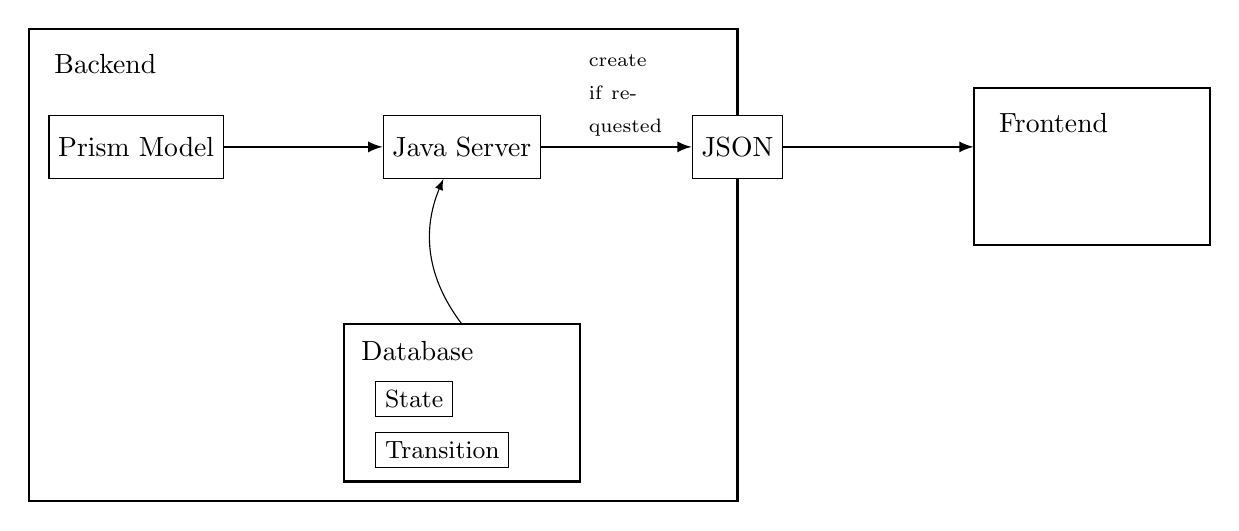
\begin{tikzpicture}
		\newcommand{\backendheight}{6}
		\newcommand{\backendwidth}{9}
		\newcommand{\backendvertpos}{0}
		\newcommand{\backendhorpos}{0}
		\newcommand{\frontendvertpos}{3.25}
		\newcommand{\frontendhorpos}{12}
		\newcommand{\frontendheight}{2}
		\newcommand{\frontendwidth}{3}
		\newcommand{\labelbackenddistline}{.2}
		\newcommand{\labelfrontenddistline}{.2}
		\newcommand{\prismvertposrelativebackend}{4.5}
		\newcommand{\prismhorposrelativebackend}{.25}
		\newcommand{\javavertposrelativebackend}{4.5}
		\newcommand{\javahorposrelativebackend}{5.5}		
		\newcommand{\jsonvertposrelativebackend}{4.5}		
		\newcommand{\jsonhorposrelativebackend}{0}		
		\newcommand{\dbvertposrelativebackend}{.25}		
		\newcommand{\dbhorposrelativebackend}{4}
		\newcommand{\dbheight}{2}
		\newcommand{\dbwidth}{3}
		\newcommand{\labeldbdistline}{.1}
		\newcommand{\statevertposrelativedb}{1.05}
		\newcommand{\statehorposrelativedb}{.4}
		\newcommand{\transvertposrelativedb}{.4}
		\newcommand{\transhorposrelativedb}{.4}
		\newcommand{\dbhorpos}{\backendhorpos+\dbhorposrelativebackend}		
		\newcommand{\dbvertpos}{\backendvertpos+\dbvertposrelativebackend}		
		\draw[thick] (\backendhorpos, \backendhorpos) rectangle (\backendhorpos+\backendwidth, \backendvertpos+\backendheight);
		\draw[thick] (\frontendhorpos,\frontendvertpos) rectangle (\frontendhorpos+\frontendwidth,\frontendvertpos+\frontendheight);
		\node[minimum height=.8, anchor=north west] at (\backendhorpos+\labelbackenddistline,\backendvertpos+\backendheight-\labelbackenddistline) {Backend};
		\node[minimum height=.8, anchor=north west] at (\frontendhorpos+\labelfrontenddistline,\frontendvertpos+\frontendheight-\labelfrontenddistline) {Frontend};
		\node [gstate, anchor= west] (prism)at (\backendhorpos+\prismhorposrelativebackend, \backendvertpos+\prismvertposrelativebackend) {Prism Model};
		\node [gstate] (java) at (\backendhorpos+\javahorposrelativebackend, \backendvertpos+\javavertposrelativebackend) {Java Server};
		\node [gstate, fill=white] (json) at (\backendhorpos+\backendwidth+\jsonhorposrelativebackend, \backendvertpos+\jsonvertposrelativebackend) {JSON};
		\draw[thick] (\backendhorpos+\dbhorposrelativebackend, \backendhorpos+\dbvertposrelativebackend) rectangle (\backendhorpos+\dbhorposrelativebackend+\dbwidth, \backendvertpos+\dbvertposrelativebackend+\dbheight);
%		\node [gstate, minimum height=7, minimum width=4] (db) at (\dbhorposrelativebackend, \dbvertposrelativebackend) {};
		

		\node (db) at (\javahorposrelativebackend, \backendvertpos+\dbvertposrelativebackend+\dbheight) {};
		
		\path [trans] (prism) edge node [midway] (prismjava) {} (java);
		\path [trans] (json) edge node [midway] (jsonfrontend) {}  ++(right:\frontendhorpos-\backendhorpos-\backendwidth);
		\path [trans] (java) edge node [midway,above,text width=.7cm] (jsonfrontend) {\scriptsize create if requested} (json);
%		\path [bendtrans] (java) edge ++(down:\javavertposrelativebackend-\backendvertpos-\dbvertposrelativebackend-\dbheight-0.4); % 0.4 because minsize gstate=0.8
%		\path [bendtrans] (java) edge node [midway] {} (db.center);
		\path [->, bend left] (db.center) edge node [midway] {} (java);
		
		\node [anchor=north west] at (\backendhorpos+\dbhorposrelativebackend+\labeldbdistline,\backendvertpos+\dbvertposrelativebackend+\dbheight-\labeldbdistline) {Database};
		\node [draw, minimum size=.6, anchor=west] at (\dbhorpos+\statehorposrelativedb,\dbvertpos+\statevertposrelativedb) {\small State};
		\node [draw, minimum size=.6, anchor=west] at (\dbhorpos+\transhorposrelativedb,\dbvertpos+\transvertposrelativedb) {\small Transition};
		
%		\node at (\backendhorpos, \dbvertpos) at ()
		
		
	\end{tikzpicture}
\end{document}
	\caption{Project Structure, showing interaction and internal structure of frontend and backend}
	\label{fig:projectstructure}
\end{figure}

Views are implemented within the server on the backend side in the 
%\lstinline[breaklines=true]{prism.core.views} 
\texttt{prism.core.views} package \redcomment{lstinline doesnt work for some reason}. 
Each view is represented by a Java class. While individual views often have their own dedicated class, sometimes multiple similar views are implemented within a single class. All views inherit from the abstract class \texttt{View}. This abstract class contains common attributes and methods required by all views. Many of these are used for testing and I/O. In listing \ref{lst:classview} an overview of relevant attributes and methods is shown. The method is \texttt{buildView()} is of particular importance as it computes the mappings of the grouping function and updates the corresponding state table in the database. The process involves 1) checking prerequisites, 2) creating a new column for storing grouping results, 3) applying the grouping function, which returns the mapped values in the form of a list of SQL queries and 4) executing these SQL queries to insert the computed values (see listing listing \ref{lst:buildview}).
\newcommand{\commentcolor}{\color{green!60!black}}
\newcommand{\commentcolorize}[1]{{\commentcolor#1}}

\lstdefinestyle{javaStyle}{
	language=Java,
	basicstyle=\small\ttfamily,
	keywordstyle=\color{blue}\bfseries,
	commentstyle=\commentcolor,
	stringstyle=\color{purple},
	numbers=left,
	numberstyle=\tiny\color{gray},
	stepnumber=1,
	numbersep=8pt,
	backgroundcolor=\color{gray!10},
	showspaces=false,
	showstringspaces=false,
	showtabs=false,
	frame=single,
	tabsize=4,
	captionpos=b,
	breaklines=true,
	breakatwhitespace=false,
%	escapeinside={\%*}{*)}
	escapechar=\~
}

%
%\lstdefinestyle{intellij}{
%	backgroundcolor=\color{intellijbg},
%	basicstyle=\ttfamily\small,
%	commentstyle=\color{intellijcomment},
%	keywordstyle=\color{intellijkeyword},
%	stringstyle=\color{intellijstring},
%	frame=single,
%	framerule=0pt,
%	showstringspaces=false,
%	numbers=left,
%	numberstyle=\tiny\color{gray},
%	breaklines=true,
%	breakatwhitespace=true,
%	captionpos=b,
%	tabsize=4,
%	columns=fullflexible,
%	keepspaces=true,
%	escapechar=\!
%}


%\lstset{
%	tabsize = 4, %% set tab space width
%	showstringspaces = false, %% prevent space marking in strings, string is defined as the text that is generally printed directly to the console
%	numbers = left, %% display line numbers on the left
%	commentstyle = \color{green}, %% set comment color
%	keywordstyle = \color{blue}, %% set keyword color
%	stringstyle = \color{red}, %% set string color
%	rulecolor = \color{black}, %% set frame color to avoid being affected by text color
%	basicstyle = \small \ttfamily , %% set listing font and size
%	breaklines = true, %% enable line breaking
%	numberstyle = \tiny,
%}


%\begin{minipage}{.94\textwidth}
	\begin{lstlisting}[style=javaStyle, caption={Most relevant attributes and methods of class \texttt{View}}, label={lst:classview}]
public abstract class View implements Namespace {
	
	protected final ViewType type;
	
	protected final Model model;
	
	protected long id; 
	
	protected Set<Long> relevantStates; 
	// refers to ~$\commentcolorize{\smstates}$~ from ~\commentcolorize{\viewN}~ definition (default: ~\commentcolorize{$\smstates := \states$}~)
	
	protected Map<String,Set<String>> stateRestriction 
										   = new HashMap<>();
	// refers to ~\commentcolorize{$Z$}~ from Definition 
	// used to determine relevantStates
	
	protected boolean semiGrouping = true; ~\commentcolorize{$\remelem \in {\grpfct}[\states]$ allowed}~
	// true: remaining states without property grouped
	// false: remaining states without property NOT grouped
	
	protected enum BinaryMode {SHOW, HIDE} // ~\commentcolorize{$\disregardelem \in \{\hasppty, \notppty\}$}~
	// HIDE: Group states that have the property 
	// SHOW: Group states that do NOT have the property
	
	protected BinaryMode binaryMode = BinaryMode.SHOW;
	// declares binary mode, only queried in binary ~\commentcolorize{\viewsN}~
	
	private void setRelevantStates(Map<String, Set<String>> stateRestriction) { ~\commentcolorize{...}~ }
	
	public void buildView() { ~\commentcolorize{...}~ }
		
	protected abstract List<String> groupingFunction() throws Exception;
	// function that performs the logical part of buildView()
	// returns list of sql statements that write the assigned value to the database
	

\end{lstlisting}
%\end{minipage}
%\begin{minipage}{.06\textwidth}
%\end{minipage}
	
%\begin{minipage}{.02\textwidth}
%\end{minipage}
%\begin{minipage}{.94\textwidth}
	\begin{lstlisting}[style=javaStyle, caption={Implementation of \texttt{buildView() function}}, label={lst:buildview}]
public void buildView() {
	try {	
		// 1. View specific checks
		if (!viewRequirementsFulfilled()) return;
					
		// 2. Create new Column 
		model.getDatabase().execute(String.format("ALTER TABLE %s ADD COLUMN %s TEXT DEFAULT %s",
		model.getStateTableName(), getCollumn(), Namespace.ENTRY_C_BLANK));
		
		// 3. Compute grouping function mapping
		List<String> toExecute = groupingFunction();				
		// 4. Write mapping to database
		model.getDatabase().executeBatch(toExecute);
		
	} catch(Exception e){
		throw new RuntimeException(e);
	}		
}

\end{lstlisting}

%\end{minipage}	
%\begin{minipage}{.06\textwidth}
%\end{minipage}
%	\begin{lstlisting}[language = Java , frame = trBL , firstnumber = last , escapeinside={(*@}{@*)}]
%		public class Factorial
%		{
%			public static void main(String[] args)
%			{   final int NUM_FACTS = 100;
%				for(int i = 0; i < NUM_FACTS; i++)
%				System.out.println( i + "! is " + factorial(i));
%			}
%			
%			public static int factorial(int n)
%			{   int result = 1;
%				for(int i = 2; i <= n; i++) (*@\label{for}@*)
%				result *= i;
%				return result;
%			}
%		}
%	\end{lstlisting}



Creating a new view entails implementing the grouping function, the method \texttt{getCollumn()} , and any necessary private attributes. This approach matches the formal definition of \viewsN and ensures consistency in the process of generating \viewsN, given that each view is essentially defined by its grouping function.

Parallel composition of views is achieved by simply creating another view, resulting in the grouping function entries being written to a new column in the database. Selective composition involves setting a  restriction that corresponds to $Z$ from Definition \ref{def:compositionselective}. This restriction is realized with a map, mapping column names to lists of allowed values. In contrast to the formalization this restriction is then used to generate an SQL Query, that selects states from the database that meet this requirement. This is achieved by setting the where clause of the SQL statement to a boolean formulae in conjunctive normal form that expresses the requirement.

The concept of disregarding views is implemented a little less general as in the formalization. In this context, the variable "semigrouping" plays a crucial role, indicating whether something should be grouped or not. For categorizing views disregarding the disregarded value is fixed empty set or string. That is, only for states that would otherwise be mapped to an empty set or string, it can be set whether they are to be grouped. For instance, in the case of the \viewN \viewscc with a parameter "n" equal to 3, the variable "semigrouping" determines whether states in an \sccN with less than three states are grouped together. For binary views, an enumeration value decides whether \hasppty or \notppty should possibly be disregarded (not grouped), in the case of the variable "semigrouping" being true.

To create a view, one accesses \nolinkurl{localhost:8080/<model\_id>/view:<viewname>?param=<param\_val\_1>\&param=<param\_val\_2>..."} via a browser, assuming the backend and frontend are operational. Afterward, accessing \nolinkurl{localhost:3000/?id=<model\_id>/} displays the graphical \viewN representation. The accessing of \nolinkurl{localhost:8080} causes the call of \texttt{createView()}, which creates a new view by calling its constructor, saves it in the internal list of views and finally calls \texttt{build()} on it, which causes the the grouping function values of the view being written to the database. When accessing \nolinkurl{localhost:3030} the frontend calls the backend which then creates and provides the JSON file to the frontend with the information stored in the database. This includes the saved information about the grouping function mappings.

The implementation of views utilizes an internal graph structure that was particularly essential for views that employ grouping based on the structural properties of the MDP graph. To facilitate this, the application utilizes the \jgrapht library \cite{Michail2020}, which not only provides graph structures but also offers many common graph algorithms. This library was selected because it is the most common, most up to date java library for graphs with the best documentation and broadest functionality. The MDP itself is represented by the class MdpGraph that inherits from the class \texttt{DirectedWeightedPseudgraph} from the \jgrapht library. A directed weighted pseudograph has been chosen because it is directed, allows weights, self loops and multiple edges between nodes, as they occur in \chgphsN, where the weights are set to the transition probabilities, edges are transitions and nodes are states.

To maintain a lightweight graph, nodes and vertices are represented as long values, referring to state and transition IDs. Information about states and transitions is accessible via hashmaps within the \texttt{MdpGraph} class. These hashmaps facilitate modular access to essential information for view functionalities.

Apart from implementation of \viewsN and by them required classes and data structures, several functionalities have been implemented to allow the following actions at runtime without restarting the server: \redcomment{based on code, link to artefact}
\begin{itemize}
	\item Display current \viewN information (Parameter values etc.) and built views
	\item Rebuild \viewN with new parameters
	\item Remove views by providing id or name		
\end{itemize}

These rely on several string parsing methods that have been implemented.





\end{document}